\documentclass[a4paper,12pt,landscape]{book}

\usepackage{ctex}
\usepackage{fontspec}

\usepackage[a4paper,inner=1.7cm,outer=2.7cm,top=2cm,bottom=2cm,bindingoffset=1.2cm]{geometry}
\usepackage[scaled=0.92]{helvet}

\usepackage[english]{babel}
\usepackage{blindtext}

\usepackage{microtype}
\usepackage{graphics}
\usepackage{wrapfig}
\usepackage{enumitem}
\usepackage{fancyhdr}
\usepackage{amsmath}
\usepackage{index}
%\usepackage{paralist}
\makeindex

\newcommand{\NTT}{New Think Tank}
\newcommand{\NTTB}{\textbf{New Think Tank}}
\newcommand{\typew}[1]{\texttt{#1}}
%清空空白页
\let\cleardoublepage\clearpage
\begin{document}
	\title{{\large \textbf{Resume}}}
	\author{foreverlz1111}
	\date{}
	\maketitle
	你好 \\
	hello \\
	你!好! \\
	% 目录
	\tableofcontents 
	
	%页号显示类型
	\pagenumbering{arabic}
	
	%页计数器 
	\setcounter{page}{3}
	
	\fancyhf{}
	\renewcommand{\headrulewidth}{2pt}
	\renewcommand{\footrulewidth}{1pt}
	\fancyhead{LE}{\leftmark}
	%\fancyhead{RO}{\nouppercase{\rightmark}}
	\fancyfoot{LE,RO}{\thepage}
	
	\chapter{章节}
	\blindmathtrue
	\blindtext[5]
	\section{版块1 图文}
	\blindtext
	\begin{figure}[ht]
		\centering
		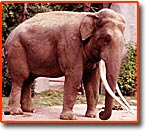
\includegraphics{elephantbig.jpg}\caption{elephan}\label{pic:elephan}
	\end{figure}
	\blindtext
	\newpage
	\section*{图片}
	\begingroup
	\setlength{\columnsep}{15pt}
	\begin{wrapfigure}{r}{.45\textwidth}
		\centering
		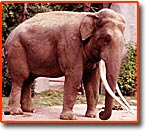
\includegraphics{elephantbig.jpg}
		\caption{图片}\label{fig:prettypic}
	\end{wrapfigure}
	\blindtext
	%必须留空一行
	
	\endgroup
	\section*{空白}
	\LaTeX\
	任意内容 \\
	空白  空白      空白 \\[10pt]
	%取消空格
	\nolinebreak
	
	\section[版块2 目录显示的名称]{文章内显示名称}
	\begin{itemize}
		\item 选择
		\item 选择
		\item 选择
		\item 选择
		\item 选择
		\begin{itemize}
			\item 选择
			\item 选择
			\item 选择
			\item 选择
			\item 选择
		\end{itemize}
			\item 选择
			\item 选择
	\end{itemize}
	
	\section{版块3 另起一页}
	\blindtext[2]
		
	% 另起一页
	\pagebreak
	\newpage
	
	\setlist{nosep}
	
	\section{版块4 item}
	\begin{enumerate}[label=\arabic*.,font=\bfseries]
		\item 选择
		\item 选择
		\begin{itemize}
			\item 选择
			\item 选择
			\item 选择
		\end{itemize}
		\item 选择
		\item 选择
				\item 选择
		\begin{itemize}
			\item 选择
			\item 选择
			\item 选择
		\end{itemize}
		\item 选择
		\item 选择
	\end{enumerate}
\bigskip

\begin{description}
	\item [选择1]解释文本
	\item [选择2]解释文本
	\item [选择3]解释文本
	\item [选择4]解释文本
	\item [选择5]解释文本
	\item [选择6]解释文本
\end{description}

\begin{tabbing}
	标题 \= 姓名 \hspace{1.5cm}\=昵称\hspace{1.5cm} \=备注\hspace{1.5cm}\\
	\> 文本 \>  文本 \> 文本\\
	\> 文本 \>  文本 \> 文本\\
	\> 文本 \>  文本 \> 文本\\
\end{tabbing}

\begin{table}
		% l居左 c居中 r居右
\begin{tabular}{lllll}
	\textbf{文本}&\textbf{文本}&\textbf{文本}\\
	\hline
	文本 & \verb|\emph{文本}| & \emph{文本} \\
	文本 & \verb|\textit{文本}| & \textit{文本} \\
	文本 & \verb|\textbf{文本}| & \textbf{文本} \\
	文本 & \verb|\texttt{文本}| & \texttt{文本} \\
	文本 & \verb|\textsc{文本}| & \textsc{文本} \\
	文本 & \verb|\textsf{文本}|{文本}|& \textsf{文本} \\
	文本 & \verb*|\underline{文本}| & \underline{文本} \\	
\end{tabular}
\caption{表格名}\label{sec:typeemp1}
\end{table}

\begin{tabular}{@{}*3l@{}}
	
	%			占两个格、居中、文本内容
	\multicolumn{2}{c}{文本1}&
	
	\multicolumn{1}{c}{文本2} \\
	first & last \\
	\hline
	文本 & 文本 & 12 \\
	文本 & 文本 & 12 \\
	文本 & 文本 & 12 \\
\end{tabular}

\section[版块5 各式各样文本]{\textsf{版块5 各式各样文本}}
\label{sec:typeemp2}
\itshape 文本,\slshape 文本
{\large 文本}{\Large 文本}{\Large 文本}{\LARGE 文本}{\huge 文本}{\Huge 文本}
\begin{LARGE}
	这里是大大的内容...
\end{LARGE}
\begin{quote}
	引用内容 \\
	引用内容 \\ 引用内容 \ 引用内容
\end{quote}

\section{版块6 数学公式}
	\begin{flalign*}
		ax^2 + bx + c = 0
	\end{flalign*}
这个公式 \( ax^2 + bx + c = 0 \) 显示 \\
$ (\cos ^{2} 30 ^{o} - \! 1)^{2} $ \\
计算以下题目:$ \frac{\sqrt{x^{3}-9}}{\sqrt{y^{2}-4}} $\\
$\alpha$ \\
$\beta$ \\
显示矩阵: $ \begin{pmatrix}
	1 & 2 \\
	3 & 4
\end{pmatrix} $ \\
积分:$ \Delta x = \int_{y_{0}}^{y_{9}}v(t)dt $ \\
极限:$ \lim_{x\to0} \frac{1}{x}=\infty $ \\
求和:$ e^e + \sum_{n=0}^{\infty}\frac{x^{2}}{x!}$

\section{版块7 新命令}
\NTT or \NTTB or \typew{文本文本}
\section{版块8 文本栏}
{\centering 居中文本 \\}

\quad\parbox{12cm}{框体框体框体框体框体框体框体框体框体框体框体框体框体框体框体框体}
\quad\parbox{4cm}{\blindtext[1]}
\quad\parbox{4cm}{\blindtext[1]} \\
\quad\parbox{4cm}{\blindtext[1]} \\
\begin{minipage}{12cm}
	\blindtext[1] 
\end{minipage} \\
\blindtext[1] 
\section{版块9 页足注释}
\blindtext[1] \\ 

解释\footnote[1]{解释:一种语言构造方式,有一个 \ref{sec:typeemp1} 表格他在,第{\pageref{sec:typeemp1}}页} \\
大象图片\footnote{\ref{pic:elephan},在第{\pageref{pic:elephan}}页}\\
参照网站\cite{网站} \\
\index{索引}[参照索引] \\
\blindtext[1]\\
\clearpage
\addcontentsline{toc}{chapter}{index}
\printindex
\begin{thebibliography}{book}
	\bibitem{网站}文本内容\emph{文本}
\end{thebibliography}

\end{document}